\documentclass[sigconf]{acmart}
% defining the \BibTeX command - from Oren Patashnik's original BibTeX documentation.
\def\BibTeX{{\rm B\kern-.05em{\sc i\kern-.025em b}\kern-.08emT\kern-.1667em\lower.7ex\hbox{E}\kern-.125emX}}
% Remove the annoying stuff
\settopmatter{printacmref=false} % Removes citation information below abstract
\renewcommand\footnotetextcopyrightpermission[1]{} % removes footnote with conference information in first column
\pagestyle{plain} % removes running headers

\usepackage{Nikolai}

\usepackage{lipsum}





\begin{document}

%
% The "title" command has an optional parameter, allowing the author to define a "short title" to be used in page headers.
\title{CMIS Hand-in 2: Finite Difference Methods 2}

\author{Nikolai Plambech Nielsen}
\email{lpk331@alumni.ku.dk}
\affiliation{%
  \institution{Niels Bohr Institute, University of Copenhagen}
}


\maketitle

\section{Introduction}


\section{Semi-Lagrangian implicit time integration: solving the advection equation}
In this problem we encounter the advection equation:
\begin{equation}\label{key}
	\frac{D \phi}{D t} = (\V{u} \D \grad) \phi + \diff{\phi}{t}
\end{equation}
Where $ D\phi/Dt $ is the particle derivative of the scalar field $ \phi $, and $ \V{u} $ is the associated velocity field. We set $ D\phi/Dt = 0 $ such that no dissipation occurs for the system:
\begin{equation}\label{key}
	 \diff{\phi}{t} = -(\V{u} \D \grad) \phi
\end{equation} 
The advection equation describes the flow of some scalar field $ \phi $ in a velocity field $ \V{u} $. This could for example describe the motion of food colouring in a pool of water. Then $ \phi $ would be the density of the food colouring molecules, whilst $ \V{u} $ would be the flow of the water in the pool.

The idea behind semi-lagrangian time integration is to use this property of the advection equation, and directly use the values of the scalar field at the previous times step. Specifically we treat our grid points as particles floating along the vector field. At a previous time, the grid point particles (to first order) were at
\begin{equation}\label{key}
	\V{x}^{t - \Delta t} = \V{x}^t - \Delta t \V{u}
\end{equation}
we then use the the value of the field at these points as the value for $ phi $ on the grid points, for the next time step:
\begin{equation}\label{key}
	\phi(\V{x}^{t}) \leftarrow \phi(\V{x}^t - \Delta t \V{u}) 
\end{equation}
The problem then, is that we are not guaranteed, that the grid point particles hit a grid point position, and as such we might not know the value of $ \phi(\V{x}^t - \Delta t \V{u}) $. To get around this we use a bilinear interpolation between the four nearest grid points to $ \V{x}^{t - \Delta t} $, and use this interpolated value as the true value.

For this problem we use a velocity field of $ \V{u} = (y, -x)^T $, corresponding to constant circular motion in the clockwise direction. For the scalar field we use a sum of Gaussian functions. If we choose the width of the Gaussians to be sufficiently small, and a large domain, virtually all the points of $ \phi $ that are non-zero will be nowhere near the boundary of the domain. This ensures that a bilinear interpolation always has enough points to use for the interpolation.

With this vector field, we expect the scalar field to rotate in time, with a period of $ 2\pi $. We can then perform an (approximate) full rotation in $ N $ steps by defining $ \Delta t = 2\pi/N $. It is only approximate due to the truncation error present when discretising the system.


\subsection{Experiments}




\section{Mean curvature flow with finite difference methods}
Next we turn our attention to solving the mean curvature flow equation for some signed distance field. Mean curvature flow is analogous to wrapping a tight string around an isosurface of a scalar field and then tightening the string such that it follows the isosurface at a higher value. The equation is given by
\begin{equation}\label{key}
	\diff{\phi}{t} = \nabla \D \frac{\nabla \phi}{||\grad \phi ||} = \kappa
\end{equation}
The right hand side of the equation can be rewritten as
\begin{equation}\label{key}
	\kappa = \frac{\grad \phi^T \grad \phi \tr H  - \grad\phi^T H \grad\phi}{||\grad\phi||^3}
\end{equation}
with $ H $ being the Hessian matrix.

\subsection{Signed Distance Fields}
A signed distance field is a scalar field describing the signed euclidian distance from each pixel of a black and white, binary image, to the nearest border between black and white, in units of pixels. The sign is such that white pixels are counted as inside, with a negative distance to the border. A one dimensional is seen in figure \textbf{INSERT REFERENCE}, where the inside is defined to be $ x \in [5, 11] $. For points sufficiently close to a border will have a gradient of approximately 1.
\begin{figure}
	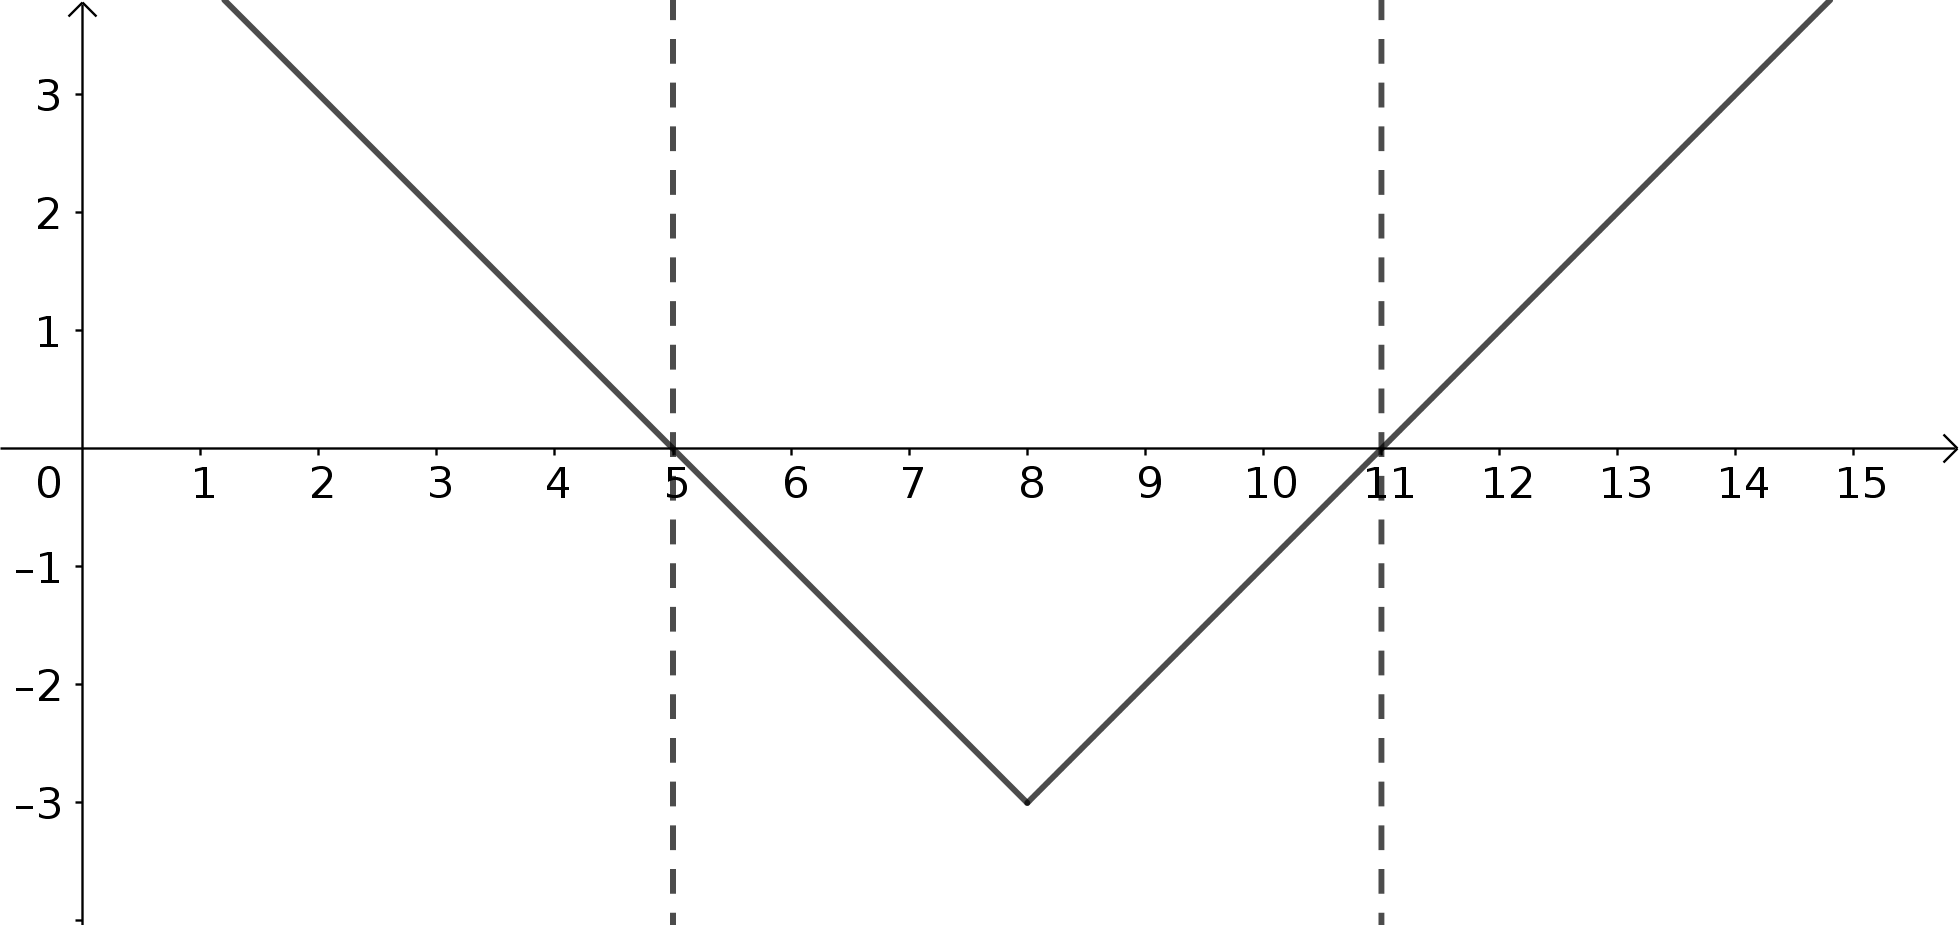
\includegraphics[width=\linewidth]{signed_distance_1d}
	\caption{A signed distance field in one dimension, with the inside as $ x \in [5, 11] $.}
	\label{fig:signed_dist}
\end{figure}


\subsection{Discretisation}
For the domain we employ a central difference approximation for each of the different spatial derivatives. This gives
\begin{equation}\label{key}
	\kappa \approx k = \frac{(D_x \phi)^2 D_{yy}\phi + (D_y \phi)^2 D_{xx}\phi - 2D_{xy}\phi D_x \phi D_y \phi}{\bb{(D_x\phi)^2 + (D_y\phi)^2}^{3/2}}
\end{equation}
where $ D $  is the central difference approximation, where the subscripts denote which variables are differentiated with respect to. For example the central difference approximation for the second order derivative with respect to $ x $:
\begin{equation}\label{key}
	D_{xx} \phi_{ij} = \frac{\phi_{i+1, j} - 2\phi_{i,j} + \phi_{i-1,j}}{\Delta x^2}.
\end{equation}
Some problems with this equation would be at or around points where the norm of the gradient disappears. This would result in possible division by zero, or just a very large value of $ k $.

A conservative maximum bound for the mean curvature is given by the inverse of the grid spacing: $ k_{\max} = \max(\Delta x, \Delta y)\inverse $. To remedy values that are too large one can clamp the value of $ k $ to between $ \pm k_{\max} $ by
\begin{equation}\label{key}
	k\leftarrow \max(-k_{\max}, \min(k, k_{\max})).
\end{equation}

For the temporal derivative we employ a first order forward difference to integrate in time:
\begin{equation}\label{key}
	\phi_{ij}^{t+\Delta t} = \phi_{ij}^t + \Delta t k_{ij}, 
\end{equation}
for some small $ \Delta t $.

This numerical scheme is conditionally stable, since too large a time step will lead to numerical blow up of the solution. The condition is called the CFL condition, and is given by
\begin{equation}\label{key}
	\Delta t \leq \frac{h}{2k_{\max}}, \quad h = \min(\Delta x, \Delta y)
\end{equation}

\subsection{Boundary conditions}
For a signed distance field, the boundary nodes will not have a fixed value, and as such a von Neumann boundary condition is preferable to a Dirichlet boundary condition. In general, the signed distance field will have a gradient of $ \pm 1 $ in each direction, so long as the node is sufficiently far away from the midpoint of a region. Since midpoints cannot occur at the boundary, it makes sense to extend the derivative to the boundary. For the left boundary this would mean $ d\phi_{1,j}/dx = d\phi{2_j}/dx$. This is implemented using ghost nodes and a central difference approximation:
\begin{equation}\label{key}
	\diff{\phi_{1,j}}{x} = \diff{\phi_{2,j}}{x} \quad \Rightarrow \quad \frac{\phi_{2,j} - \phi_{0,j}}{2\Delta x} = \frac{\phi_{3,j} - \phi_{1,j}}{2 \Delta x}
\end{equation}
Giving the updating formula for ghost nodes on the left boundary:
\begin{equation}\label{key}
	\phi_{0,j} = \phi_{1,j} + \phi_{2,j} - \phi_{3,j}.
\end{equation}

\subsection{Experiments}


\end{document}
